\documentclass[14pt]{extarticle} 
\usepackage{amsmath,mathtools,amsfonts,amsthm,amssymb,hyperref}
\usepackage{wasysym,geometry,bussproofs,latexsym,parskip,bookmark}
\usepackage{mathtools,float}
\newtheorem{defn}{Definition}
\newtheorem{thm}{Theorem}
\newtheorem{claim}{Claim}
\newtheorem{lemma}{Lemma}
\newcommand{\dps}{\displaystyle}
\hypersetup{colorlinks,allcolors=blue,linktoc=all}
\geometry{a4paper} 
\geometry{margin=0.5in}
\title{Math for CS 2015/2019 solutions to ``In-Class Problems Week 14, Wed. (Session 35)''}
\author{https://github.com/spamegg1}
\begin{document}
\maketitle
\tableofcontents

\section{Problem 1}
\subsection{(a)}
\begin{figure}[ht!]
\centering
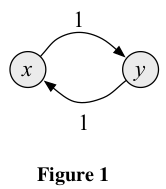
\includegraphics[scale=0.6]{random-walk-1.png}
\end{figure}
Find a stationary distribution for the random walk graph in Figure 1.
\begin{proof}
\end{proof}

\subsection{(b)}
Explain why a long random walk starting at node $x$ in Figure 1 will not converge to a stationary distribution. Characterize which starting distributions will converge to the stationary one.
\begin{proof}
\end{proof}

\subsection{(c)}
\begin{figure}[ht!]
\centering
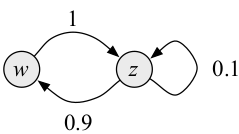
\includegraphics[scale=0.6]{random-walk-2.png}
\end{figure}

Find a stationary distribution for the random walk graph in this figure.
\begin{proof}
\end{proof}

\subsection{(d)}
If you start at node $w$ above and take a (long) random walk, does the distribution over nodes ever get close to the stationary distribution? You needn’t prove anything here, just write out a few steps and see what’s happening.
\begin{proof}
\end{proof}

\subsection{(e)}
\begin{figure}[ht!]
\centering
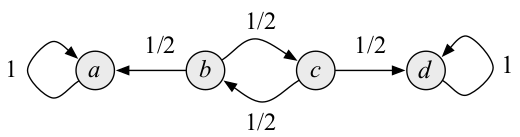
\includegraphics[scale=0.6]{random-walk-3.png}
\end{figure}
Explain why the random walk graph in this figure has an uncountable number of stationary distributions.
\begin{proof}
\end{proof}

\subsection{(f)}
If you start at node $b$ in the last figure and take a long random walk, the probability you are at node $d$ will be close to what fraction? Explain.
\begin{proof}
\end{proof}

\subsection{(g)}
Give an example of a random walk graph that is not strongly connected but has a unique stationary distribution. Hint: There is a trivial example.
\begin{proof}
\end{proof}

\section{Problem 2}
Prove that for finite random walk graphs, the uniform distribution is stationary if and only the probabilities of the edges coming into each vertex always sum to 1, namely
$$
\sum_{u \in \text{into}(v)} p(u,v) = 1
$$
where into$(w) \Coloneqq \{v\,\, | \,\,\langle v \to w\rangle \text{ is an edge}\}$.
\begin{proof}
\end{proof}

\section{Problem 3}
A Google-graph is a random-walk graph such that every edge leaving any given vertex has the same proba­bility. That is, the probability of each edge $\langle v \to w \rangle$ is 1= outdeg.v/.

A digraph is symmetric if, whenever $\langle v \to w\rangle$ is an edge, so is $\langle w \to v\rangle$. Given any finite, symmetric Google-graph, let $d(v) \Coloneqq$ outdeg$(v) / e$ where $e$ is the total number of edges in the graph.

\subsection{(a)}
If $d$ was used for webpage ranking, how could you hack this to give your page a high rank? ...and explain informally why this wouldn’t work for “real” page rank using digraphs?

\begin{proof}
\end{proof}

\subsection{(b)}
Show that $d$ is a stationary distribution.

\begin{proof}
\end{proof}

\end{document}
